\chapter{Implementation}

\section{Javascript Cryptography}

\paragraph{The developer decided that the best solution for the cryptography implementation was the utilization of a pre-existing cryptography library.}

\paragraph{For this task, there were three necessary conditions that had to be met:}

\begin{itemize}
\item A clear, easily identifiable, and reputable source/owners
\item Existing, easily obtainable, and comprehensive documentation
\item Open source, easily available code
\end{itemize}

\paragraph{and, slightly less important, actively maintained.}

\paragraph{Meeting the above criteria was not as simple as it would seem. There were many options that met some of the conditions, but meeting them all was more challenging. Ultimately, however, the researcher was satisfied with the Stanford Javascript Crypto Library (SJCL), as it met all the above conditions. Additionally, it appeared to be well developed, and maintained.}\cite[Website]{SJCL}

\paragraph{The usage is pretty straight forward, and will work for this implementation. Simply linking the javascript source in the html file (See reference figure: \ref{fig: exampleSJCL_html}).:}

\begin{figure}[H]
\begin{minted}[breaklines]{html}
<!DOCTYPE html>
<html>
<head>
    <meta charset="utf-8"/>
    <script src="http://bitwiseshiftleft.github.io/sjcl/sjcl.js"></script>
</head>
</html>
\end{minted}
\caption{\label{fig: exampleSJCL_html} Example of linking SJCL in HTML}
\end{figure}

\paragraph{and, the javascript can simply be used as follows (See reference figure: \ref{fig: exampleSJCL_js}):}

\begin{figure}[H]
\centering
\begin{minted}[breaklines]{javascript}
var ciphertext = sjcl.encrypt("reallyHardPasswordNoOneCouldEveryGuess", "Hello World!");
var plaintext = sjcl.decrypt("reallyHardPasswordNoOneCouldEveryGuess", ciphertext);
console.log("plain text: " + plaintext);
console.log("cipher text: " + ciphertext);
console.log("plain text - again!: " + plaintext);
\end{minted}
\caption{\label{fig: exampleSJCL_js} Example of javascript SJCL}
\end{figure}

\paragraph{giving the following result (See reference figure: \ref{fig: exampleSJCL}):}

\begin{figure}[H]
\centering
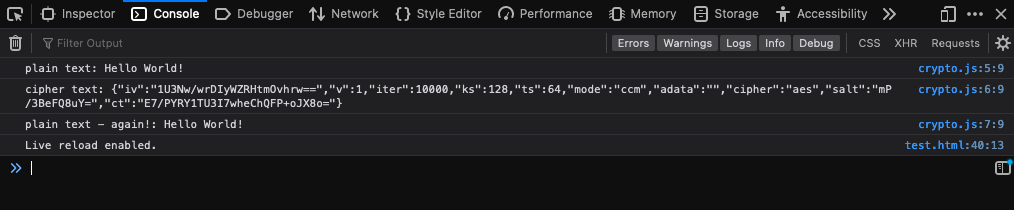
\includegraphics[width=0.9\textwidth]{exampleSJCL.png}
\caption{\label{fig: exampleSJCL} Example output to Firefox console}
\end{figure}

\paragraph{The usage is pretty straight forward, and will meet our needs.}

\section{WebExtensions}

\paragraph{WebExtensions are web technology built with the tools that are natural to any web developer: HTML, CSS, and Javascript. Each extension must have a \emph{manifest.json} file, which essentially hold all the vital information as to the author of the software, permissions required to use the add-on, the software version, and so on.} \cite[Webpage]{WebEx}

\paragraph{Starting with the release of Thunderbird version 68 (August 2019), Thunderbird moved to only support WebExtensions for add-ons and themes development, with all previous versions no longer working. Even the long standing Enigmail cryptography add-on that the author used for years, no longer functioned.}

\paragraph{Here is an image from Mozilla's Thunderbird Add-on Webpage that gives a quick glance of how the extensions might look like.}\footnote{Source: same webpage as noted above.}


\begin{figure}[H]
\centering
\includegraphics[width=0.9\textwidth]{webEx.png}
\caption{\label{fig: webEx} WebExtension overview}
\end{figure}


\section{Implementation Details}
\paragraph{But, lets dive right in and get started. As we step through the development, it will become more clear.}

\subsection{Creating a button}

\paragraph{First, we'll create a button that will appear in the "Compose Window," the window that appears when you start to write an email.}

\paragraph{Before add-on implementation:}

%add image here
%add Image
\begin{figure}[H]
    \centering
    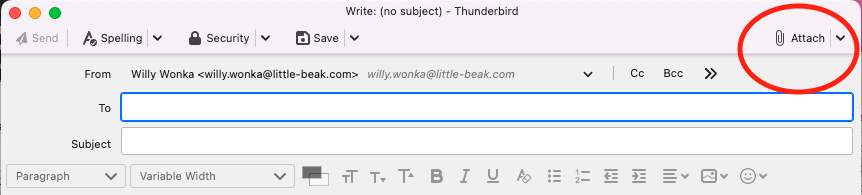
\includegraphics[width=0.9\textwidth]{ComposeWindow_No_Button.png}
    \caption{\label{fig: noButton} Normal compose window}
\end{figure}

\paragraph{with add-on button implemented.}

%add image
%add Image
\begin{figure}[H]
    \centering
    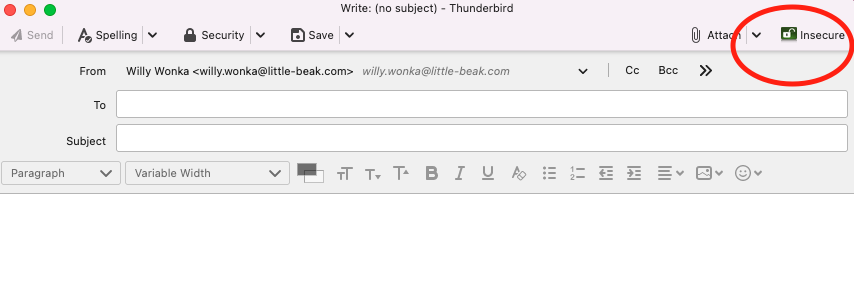
\includegraphics[width=0.9\textwidth]{ComposeWindowButtonInsecure.png}
    \caption{\label{fig: withButton} Button added to the compose window.}
\end{figure}

\paragraph{And, here is the manifest.json file that was created for this button. Most of the references in the manifest.json file, are, well manifest. The only thing of interest is the manifest version of 2. Apparently, it has to be 2, and it always is 2. The rest provide information about the add-on, location of images used, and the permissions required for the add-on to function. (See reference figure: \ref{fig: basic_manifest.json}).:}

%add code here
\begin{figure}[H]
\centering
\begin{minted}[breaklines]{javascript}
{
    "manifest_version": 2,
    "name": "Crypto add-on",
    "description": "A password AES cryptographic addon",
    "version": "1.0",
    "author": "Esteban Licea",
    "applications": {
        "gecko": {
            "id": "esteban@little-beak.com",
            "strict_min_version": "78.0"
        }
    },
    "compose_action": {
        "default_title": "Insecure",
        "default_icon": "images/unlocked_64px.png"
    },
    "permissions": [
        "menus"
    ],
    "icons": {
        "64": "images/unlocked_64px.png",
        "32": "images/unlocked_32px.png",
        "16": "images/unlocked_16px.png"
    }
}
\end{minted}
\caption{\label{fig: basic_manifest.json} Basic manifest.json file}
\end{figure}

%% I was preoccupied with the 

\subsection{Prompt for password}

\paragraph{Now that we got a working button, we're going to make it ask for a password when it's clicked. Which is simple enough by altering adding to our manifest file, and some basic Javascript. }

%add code here
\begin{figure}[H]
\centering
\begin{minted}[breaklines]{javascript}
{
    "compose_action": {
        "default_popup": "passwordPrompt/passwordPrompt.html",
        "default_title": "Insecure",
        "default_icon": "images/unlocked_64px.png"
    },
}
\end{minted}
\caption{\label{fig: addPwToManifest} Add a Password Prompt to manifest file}
\end{figure}

add code here
\begin{figure}[H]
\centering
\begin{minted}[breaklines]{javascript}
{
var user = prompt("Please enter a secure password or phrase (the longer the better): ");
if (user != null) {
    document.getElementById("greeting").innerHTML = "Greetings, " + user + "!";
}
}
\end{minted}
\caption{\label{fig: pwPrompt} Javascript prompt for password}
\end{figure}

\paragraph{To get a better understanding of our development, here is a glance at our file structure so far.}

%add Image
\begin{figure}[H]
    \centering
    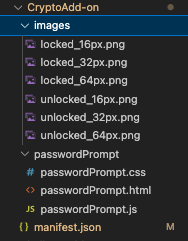
\includegraphics[width=0.6\textwidth]{fileStructureSoFar_1.png}
    \caption{\label{fig: folderStructure1} Development so far...}
\end{figure}



\subsection{Encrypt}
\subsection{Send message}

% 1) create button in the compose window - I have done this..

% 2) clicking on button does the following:
% 	gets all the content in the compose window
%	put it into a variable
%	encrypts it

% 3) once encrypted -> sends it as well?? That would be best, so need
% 	to make it such that the button reads: "Send encrypted"

% 4) 

